\documentclass{report}
\usepackage[portuges]{babel}
\usepackage[utf8]{inputenc}
\usepackage{color}
\usepackage[dvipsnames]{xcolor}
\usepackage[hidelinks]{hyperref}
%\usepackage[latin1]{inputenc}
\usepackage{float}
\usepackage{graphicx}
\usepackage{url}
\usepackage{enumerate}
\usepackage[nottoc,numbib]{tocbibind}
\usepackage{alltt}
\usepackage{fancyvrb}
\usepackage{listings}
\usepackage{amsmath}
%LISTING - GENERAL
\usepackage{xspace}
\usepackage{xcolor}
\usepackage{minted}
%\usepackage{hyperref}
%\usepackage{python}

\setcounter{secnumdepth}{3}
\setcounter{tocdepth}{3}

\definecolor{dkgreen}{rgb}{0,0.6,0}
\definecolor{dred}{rgb}{0.545,0,0}
\definecolor{dblue}{rgb}{0,0,0.545}
\definecolor{lgrey}{rgb}{0.9,0.9,0.9}
\definecolor{gray}{rgb}{0.4,0.4,0.4}
\definecolor{darkblue}{rgb}{0.0,0.0,0.6}

\parindent=4em
\parskip=2pt

\setlength{\oddsidemargin}{0.5cm}
\setlength{\textwidth}{15cm}
\setlength{\headsep}{-1cm}
\setlength{\textheight}{23cm}

\renewcommand{\baselinestretch}{1.5}
\setlength{\parindent}{4em}
\setlength{\parskip}{1em}



\lstset{
  basicstyle=\ttfamily,
  columns=fullflexible,
  showstringspaces=false,
  tabsize=4,
  commentstyle=\color{gray}\upshape
}


\title{\Large{\textbf{Engenharia de Segurança}} \\[1cm]
 \LARGE{\textbf{Trabalho Prático 3}}
\author{ Afonso Fontes\\ \small(pg35389) \and Bruno Carvalho\\ \small(a67847) \and Mariana Carvalho\\ \small(a67635)}
\date{\today\\Universidade do Minho}}


\begin{document}

\maketitle

\section*{TOR (The Onion Router)}

\subsection*{Pergunta P1.1}
\subsubsection*{Efetuando o comando \textbf{sudo anonsurf start} consegue garantir que está localizado nos EUA?}
Não, apenas conseguimos, através do comando \textbf{sudo anonsurf change} obrigar o calculo de um novo circuito que muito provavelmente tem um novo \textbf{OR} de saída, no entanto, utilizando o \textbf{anonsurf} é impossível garantir que este esteja localizado nos EUA.
 
\subsubsection*{Porquê? Utilize características do protocolo TOR para justificar.}
Isto acontece devido à forma como são seleccionados os três \textbf{ORs} fornecidos ao \textbf{OP} pelo \textbf{Directory Server}, que devem ser sempre alterados uma vez por minuto. Através do software utilizado é impossível garantir que os \textbf{ORs} seleccionados se encontram nos EUA, no entanto caso o software fosse implementado por nós, o protocolo prevê a possibilidade de utilizar circuitos escolhidos de forma não aleatória, sendo que poderiamos escolher a utilização de \textbf{ORs} localizados nos EUA para formação do nosso circuito.

\subsection*{Pergunta P1.2}
\subsubsection*{Clique no símbolo do Onion(cebola) do lado esquerdo da barra de URL e verifique qual é o circuito para esse site.}
Podemos visualizar na fig\ref{img1} e fig\ref{img2} o resultado obtido aquando da consulta do circuito para os sites correspondentes.

\begin{figure}[H]
  \centering
    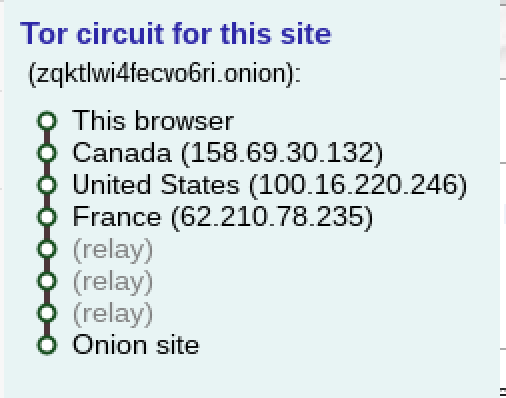
\includegraphics[width=1\textwidth]{imgs/img1}
  \caption{\textit{TOR circuit} para o primeiro site}
  \label{img1}
\end{figure}

\begin{figure}[H]
  \centering
    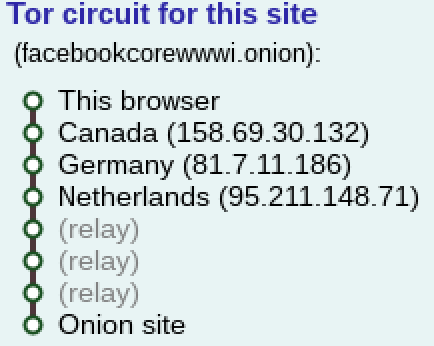
\includegraphics[width=1\textwidth]{imgs/img2}
  \caption{\textit{TOR circuit} para o segundo site}
  \label{img2}
\end{figure}


\subsubsection*{Porque existem 6 "saltos" até ao site Onion, sendo que 3 deles são "relay"? Utilize características do protocolo TOR para justificar.}
Na rede TOR, a disponibilização de serviços anónimos permite a um OP disponibilizar serviços TCP sem revelar o seu endereço IP, isto é feito pela rede TOR através de pontos de rendezvous. Em suma o que acontece é que a entidade que deseja prestar o serviço (identificada pela sua chave pública) cria um circuito cujo último(s) OR(s) denominam-se por \textit{introduction points} e são anunciados no \textit{Directory Server}. Quando nós (cliente) tentamos aceder ao serviço, obtemos informação sobre os \textit{introduction points} para o mesmo, mantendo total anonimato do serviço ao qual pretendemos aceder , ao mesmo tempo criamos um circuito até a um \textit{OR} que vai ser utilizado como o nosso \textit{Rendezvous Point}. De seguida o cliente entrega um segredo a um dos \textit{introduction points} para o serviço requisitando o mesmo através do \textit{Rendezvous Point} estabelecido, finalmente o serviço conecta-se ao \textit{RP} do cliente fornecendo o respetivo segredo. A partir de agora o cliente utiliza o circuito conhecido que acaba no \textit{RP} respetivo, garantindo anonimato até a um ponto de introdução para um circuito \textit{relay}, que proporciona anonimato ao serviço Onion que pretendemos utilizar. 



\end{document}
